\section{Planering och genomförande}
% TODO: Kort och orienterande om hur ni tänkte genomföra uppgiften. 
%       Orienterande om Planering och Genomförande.

\subsection{Planering}
% Hur kommer ni att arbeta?  Detta är en lite längre text än den rent
% orienterande texten i Planering och genomförande ovan.  För att infoga
% hänvisningar till andra delar av dokumentet hittar ni under menyn
% ”Infoga/Korshänvisning...”.  Där kan ni skapa referenser som ni kan använda 
% och ni kan lägga in sidnummer, kapitelnummer eller kapiteltext till en rubrik 
% eller referens.

\subsection{Genomförande}
% Här skriver ni vilka steg ni gjorde och resultatet av dem. Ni skall ha med
% information så att vi kan se hur ni har gjort, dvs beskrivande text,
% skärmdumpar, bilder etc.  Längre skärmdumpar, innehåll i relevanta filer och
% större bilder lägger ni i bilagor, som bilaga I, så att de inte tar över en
% sida själva.  
% Kommandon som ni skriver i ett skal skall skrivas i detta format, som är 
% teckenformatmall ”Exempel” i OpenOffice/LibreOffice. Detta så att de
% skiljer sig från övriga brödtext i stycket.  Detta underlättar läsningen för
% andra, som oss lärare.  
% Bilder lägger ni in med "Infoga/Bildobjekt/Från fil..." och sedan lägger ni 
% till text och numrering genom att markera bilden och sedan göra 
% "Infoga/Bildtext...".  Notera att man har det finns olika bildtext för dem
% som vill prova. I den här har jag valt illustration samt skrivit in en liten
% förklarande text.  Till bilden kan man sedan infoga en referens där man anger
% Illustration och sedan väljer önskad bild. 


\begin{figure}[htbp]
  \centering
    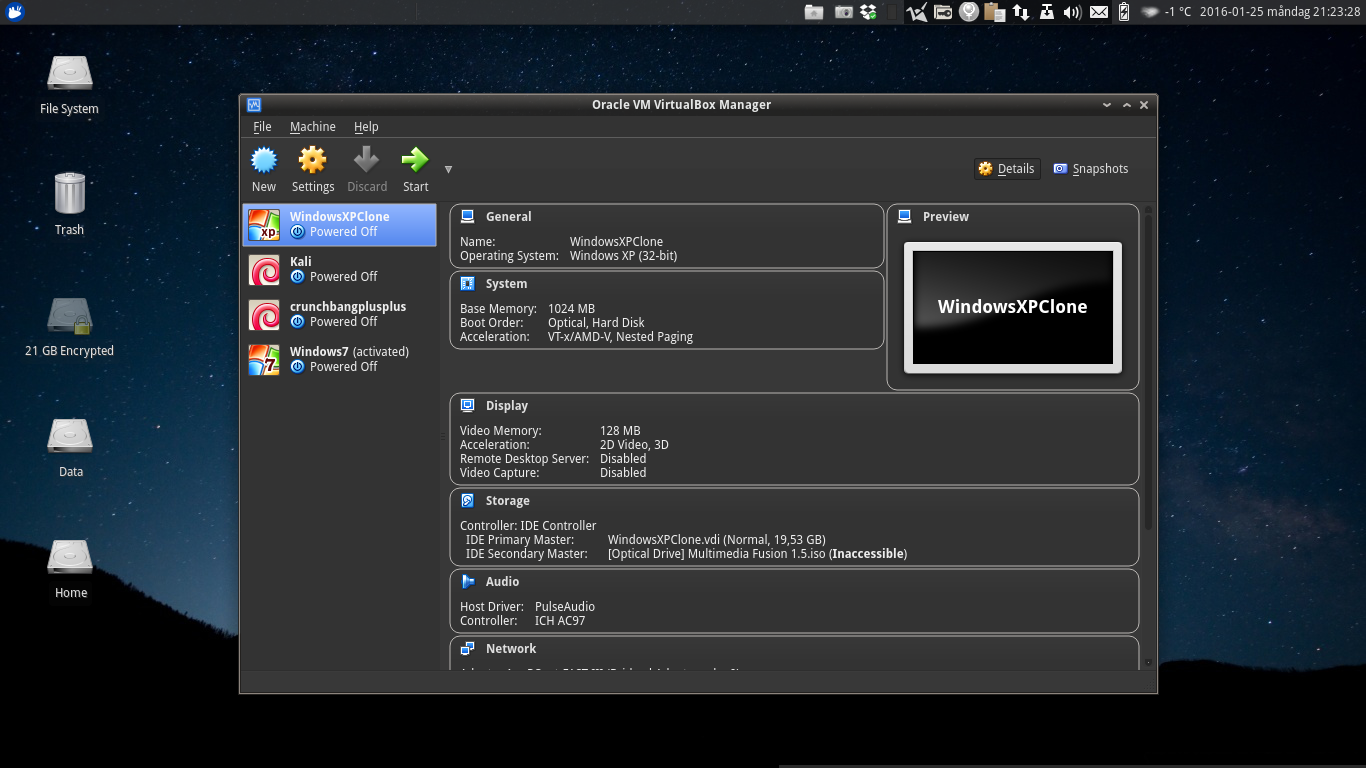
\includegraphics[width=\linewidth]{img/A_new-01}
    \caption{En ny virtuell maskin skapas i Virtualbox genom att klicka
             \texttt{New}.}
  \label{fig:A_new-01}
\end{figure}

\begin{figure}[htbp]
  \centering
    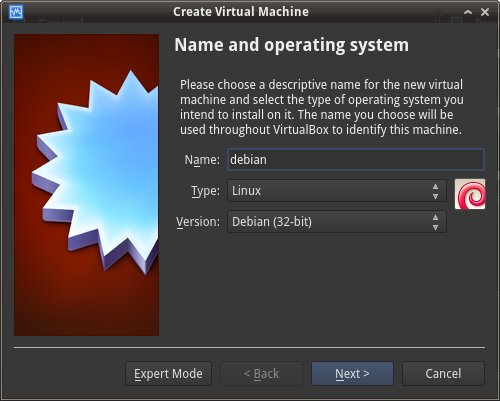
\includegraphics[width=\linewidth]{img/A_new-02}
    \caption{I dialogrutan för en ny virtuell maskin väljs namnet
             \texttt{debian} och lämplig typ samt bittal väljs automatiskt.}
  \label{fig:A_new-02}
\end{figure}

\begin{figure}[htbp]
  \centering
    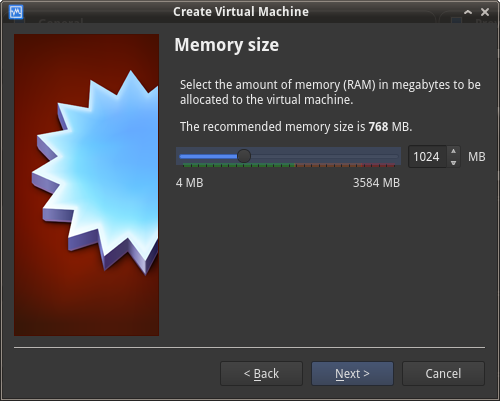
\includegraphics[width=\linewidth]{img/A_new-03}
    \caption{Storleken på RAM-minnet sätts till en lämplig kompromiss mellan
             vad värdsystemet kan tänkas behöva och vad gästsystemet kräver.}
  \label{}
\end{figure}

\begin{figure}[htbp]
  \centering
    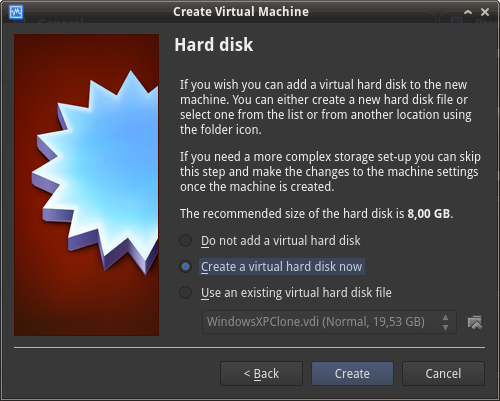
\includegraphics[width=\linewidth]{img/A_new-04}
    \caption{I dialogrutan för hårddisk väljer vi att skapa en ny virtuell
             hårddisk.}
  \label{}
\end{figure}

\begin{figure}[htbp]
  \centering
    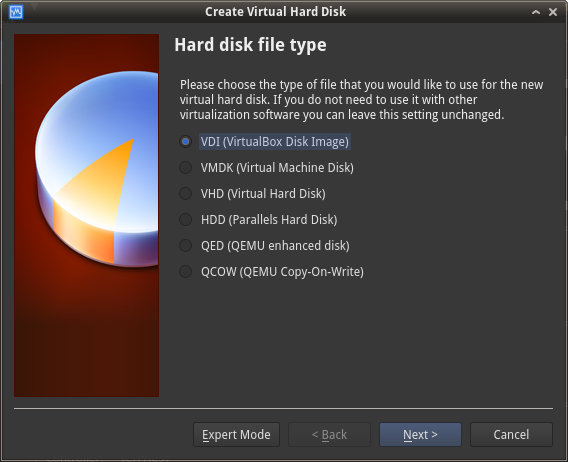
\includegraphics[width=\linewidth]{img/A_new-05}
    \caption{Standardvalet \texttt{VDI} fungerar bra för det här
             användningsområdet. Ytterigare information de olika alternativen
             finns i \cite{virtualbox:vdidetails}.}
  \label{}
\end{figure}
